\documentclass{article} % Change to the appropriate document class, i.e. report, book, article...
\usepackage{style}

\title{CSE 272 assignment 2}
\author{Alisha Lawson\\Hallgeir Lien}
\date{}
\begin{document}

\maketitle
\newpage

\section*{Introduction}
In this assignment we explore different methods of estimating the irradiance over a line in a scene. The scene used for the assignment has a rectangular diffuse area light with corners $(-1.75,-1,-0.05)$ and $(1.75,-1,0.05)$ (area $A=0.35\ m^2$) and normal $\mathbf{n_l}=(0,1,0)$ and power $\phi=100\ W$. Above the area light there is a diffuse square with corners $(-1,0,-1)$ and $(1,0,1)$ with normal $\mathbf{n_s}=(0,1,0)$. Above the square there is a mirror with corners $(-2,1,-2)$ and $(2,1,2)$ and normal $(0,-1,0)$. We estimated the irradiance over a line $AB$ between the points $A=(-1,0,0)$ and $B=(1,0,0)$ using Monte Carlo path tracing, progressive photon mapping, adaptive(Metropolis) photon mapping and Metropolis path tracing. 

\section*{Task 1}
Our first task was to estimate the irradiance using path tracing. We divided the interval between $A$ and $B$ into 100 discrete points, and from each point we shot out 10 million rays using a distribution $p(x)=\cos theta / \pi$ where $\theta$ is the angle between the normal of the diffuse surface and the direction of the ray, giving a total of 1 billion rays. Since we use a diffuse square light, the irradiance estimate becomes
$$
F(x) \approx \frac{1}{N} \sum_{i=1}^N \frac{L(x)/\pi \cos \theta}{\cos \theta / \pi} = \frac{1}{N} \sum_{i=1}^N L(x)
$$

Figure \ref{fig:pathtracing} shows the irradiance over the interval for 1 million, 10 million, 100 million and 1 billion total sample rays. The measurement points are evenly distributed between the points $A$ and $B$, with point $0$ being at point $A$ and point $99$ being at point $B$.
\begin{figure}[h]
\subfigure[1 million sample rays]{
    \includegraphics[width=0.5\textwidth]{plots/pathtracing_irrad_1mill}\\
}
\subfigure[10 million sample rays]{
    \includegraphics[width=0.5\textwidth]{plots/pathtracing_irrad_10mill}\\
}
\subfigure[100 million sample rays]{
    \includegraphics[width=0.5\textwidth]{plots/pathtracing_irrad_100mill}\\
}
\subfigure[1 billion sample rays]{
    \includegraphics[width=0.5\textwidth]{plots/pathtracing_irrad_last}\\
}
    \caption{Irradiance estimate, path tracing}
\label{fig:pathtracing}
\end{figure}

As expected, this scene requires a lot of rays in order to minimize the noise. Even after 100 million rays (1 million rays per point) there is considerable noise. If we were actually rendering an image with a similar kind of scene where we have perhaps a million pixels instead of only 100, the rendering process would take an outrageous amount of time.

The irradiance estimate seems to converte to a value of $0.72W/m^2$ near the edges, and $0.3W/m^2$ near the middle of the interval.

\section*{Task 2}
Our second task was to estimate the irradiance using Progressive Photon mapping.  We sent out 100,000 photons for 1,000 passes totaling 100 million photons emitted from the square light, which has a normal bias distribution. Initially we set the radius to $0.25$. On each pass we adjust the radius $\hat{R}(x)$ according the user-defined ratio alpha $\alpha$ set to 0.7, as
$$ \hat{R}(x) = R(x) - dR(x) = R(x)\sqrt{\frac{N(x)+\alpha M(x)}{N(x)+M(x)}}$$
Where $N(x)$ is the previously accumulated photons and $M(x)$ is the newly added photons in the current photon tracing pass for each hitpoint in the scene. Figure \ref{fig:pm_radius} shows the radius and figure \ref{fig:pm_acc} shows the number of accumulated photons over 1,000 iterations.

\begin{figure}[H]
\begin{tabular}{c}
%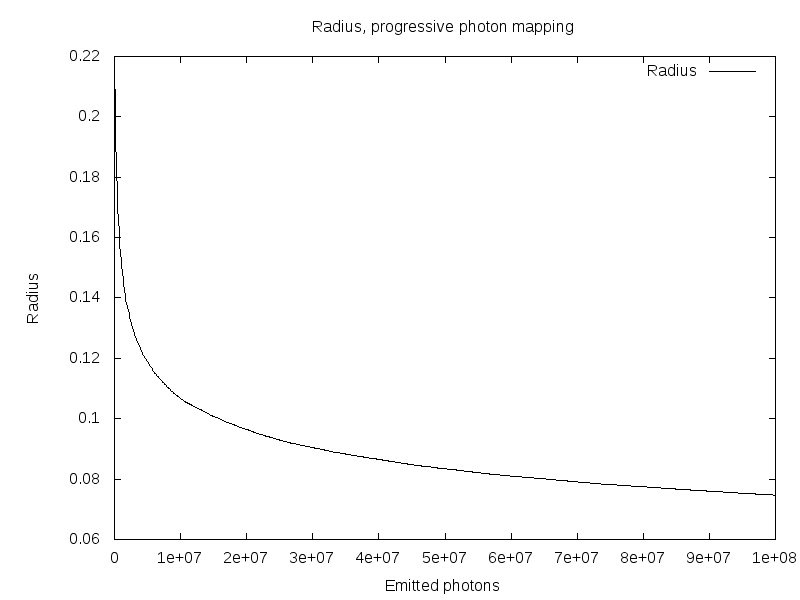
\includegraphics[width=0.9\textwidth]{plots/irrad_photonmap_radius.png}\\
\end{tabular}
\caption{Radius, photon mapping}
\label{fig:pm_radius}
\end{figure}

\begin{figure}[h]
\begin{tabular}{c}
%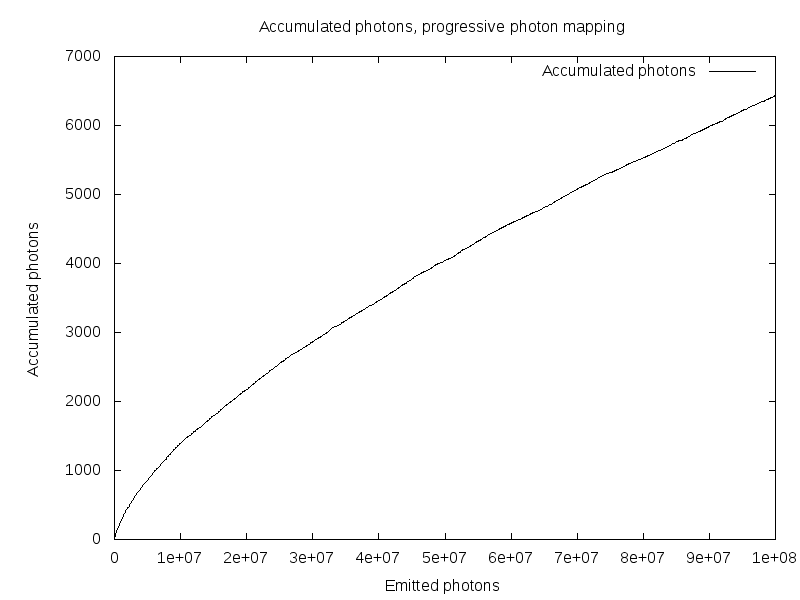
\includegraphics[width=0.9\textwidth]{plots/irrad_photonmap_photons.png}\\
\end{tabular}
\caption{Accumulated photons}
\label{fig:pm_acc}
\end{figure}

We also modify the accumulated flux $\tau_{\hat{N}}(x, \omega)$ in each pass, using
$$\tau_{\hat{N}}(x, \omega) = \tau_{N+M}(x, \omega)\frac{N(x) + \alpha M(x)}{N(x) + M(x)}$$

Since we are interested in the irradiance at point A, the BRDF does not contribute to the equation. We calculate the irradiance by normalizing $\tau_{\hat{N}}(x, \omega)$ by the number of emitted photons and the adjusted radius $\hat{R}(x)$:
$$F = \frac{\tau_{N}(x, \omega)}{\pi R(x)^2 N_{emitted}}$$

\begin{figure}[H]
\begin{tabular}{c}
%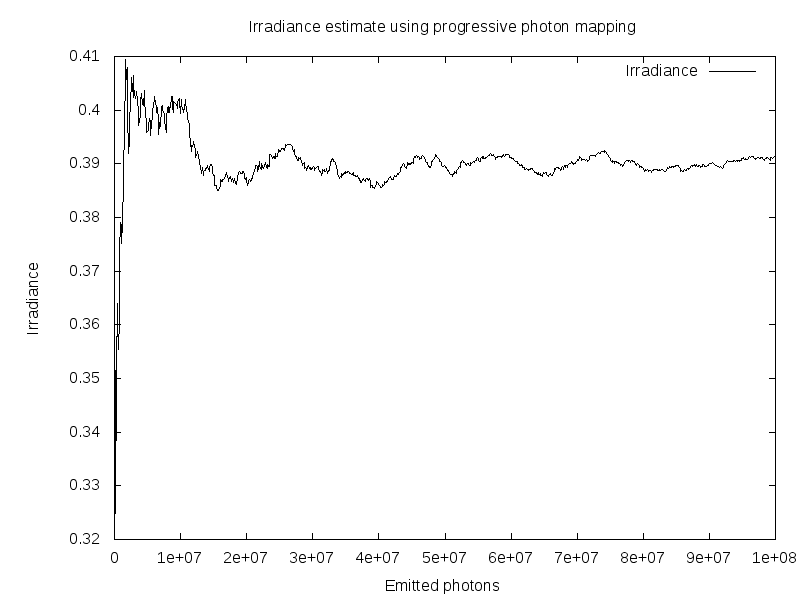
\includegraphics[width=0.9\textwidth]{plots/irrad_photonmap.png}\\
\end{tabular}
\caption{Irradiance, photon mapping}
\label{fig:pm_irradiance}
\end{figure}

%Over multiple photon tracing passes the irradiance also converges to about 0.39, as with path tracing.

\section*{Task 3 - Adaptive photon mapping}

\section*{Task 4 - Metropolis path tracing}
The last task was implementing a Metropolis light transport algorithm. A simplified view of this algorithm is that we first find a "good" path that gives a contribution. Then we slightly perturb this path, sample the new perturbed path, and either accept or reject this new path as the "good" one based on some acceptance probability $a$, and repeat. The theory is that if we do have a good path that gives a contribution $\mathbf{z}$, it's likely that a path $\mathbf{z}+\Delta \mathbf{z}$, that are perturbed by some amount $\Delta \mathbf{z}$, would also give a contribution, which allows us to more completely sample bright objects. This is often a problem for Monte Carlo path tracers because each pixel is evaluated independently which means that if there is a small bright object in the scene, one pixel may hit the object while neighboring pixels may miss it completely which introduces bright specles of noise in the image. 

Again we divide the interval into 100 discrete points. We then wish to estimate $E_i$, where $E_i$ is the irradiance for point $i$. The probability distribution of paths in Metropolis light transport is proportional to the intensities in the image, i.e. $p(\mathbf{z}) = I(\mathbf{z})/{\int I(\mathbf{z})d\mathbf{z}}$. We estimate the normalizing factor (the average intensity) 
$$
b=\int I(\mathbf{z})d\mathbf{z}\approx \frac{1}{N_s}\sum_{i=1}^{N_s} \frac{I(\mathbf{z}_i) \cos \theta_i}{\cos \theta_i/\pi} = \frac{1}{N_s}\sum_{i=1}^{N_s} I(\mathbf{z}_i)\pi
$$
by shooting $N_s$ rays from random positions with a distribution of $p = \cos \theta/\pi$. Now we use one of the paths from the seeding process as our first path $\mathbf{z}_0$. Each path $\mathbf{z}$ contibutes to one and only one point, by designating a interval of length $(1- (-1))/N_p=2/N_p$ to each point, where $N_p$ is the number of discrete points, over the full interval of length $2$. The contribution from each path is 
$$\Delta E = \frac{1}{M} \frac{I(\mathbf{z})N_p}{p(\mathbf{z})}a(\mathbf{z}_{old}\to \mathbf{z}_{new}) = \frac{1}{M} \frac{I(\mathbf{z})N_p}{I(\mathbf{z})/b} a(\mathbf{z}_{old}\to \mathbf{z}_{new}) = \frac{bN_p}{M} a(\mathbf{z}_{old}\to \mathbf{z}_{new})$$ 

where $M$ is the total number of samples. Figures \ref{fig:metropolis_irrad1}, \ref{fig:metropolis_irrad10} and \ref{fig:metropolis_irrad100} shows the irradiance estimates for the interval for 1 million, 10 million and 100 million sample rays, compared to Monte Carlo path tracing with the same number of total rays.

\begin{figure}[h]
    \centering
    \includegraphics[width=0.8\textwidth]{plots/metropolis_irrad_1mill}\\
    \caption{Metropolis vs. Monte Carlo, 1 million sample rays each}
    \label{fig:metropolis_irrad1}
\end{figure}

\begin{figure}
    \centering
    \includegraphics[width=0.8\textwidth]{plots/metropolis_irrad_10mill}\\
    \caption{Metropolis vs. Monte Carlo, 10 million sample rays each}
    \label{fig:metropolis_irrad10}
\end{figure}

\begin{figure}
    \centering
    \includegraphics[width=0.8\textwidth]{plots/metropolis_irrad_last}\\
    \caption{Metropolis, 100 million sample rays vs. Monte Carlo, 1 billion sample rays}
    \label{fig:metropolis_irrad100}
\end{figure}

We see that for this scene, the level of noise for Metropolis is significantly lower than that of Monte Carlo path tracing. Looking at the final distribution (figure \ref{fig:metropolis_irrad100}), we see that the amount of noise is about the same. However, keep in mind that the Monte Carlo used ten times as many rays to get there. The irradiance for the Metropolis run is slightly skewed (point 0 has a slightly higher irradiance than point 99); this is due to random variation. In this scene, there are two bright spots on the opposite sides of the interval, so we must rely on large steps in order to sample both sides. But even with large steps, there is a large probability that one side will be sampled more than the other.

\subsection*{Mutation strategy}
We implement the mutation strategy recommended in Csaba Kelemen et. al., "A Simple and Robust Mutation Strategy for the Metropolis Light Transport Algorithm". It's given in figure \ref{fig:mutation_metropolis}. As seen in the pseudo code, we mutate the angles by a smaller amount. This seems to work well with this scene, because when the path moves close to the middle, the solid angle of the reflected light source in the mirror is very small.

\begin{figure}[h]
\begin{algorithmic}
\STATE Let $\mathbf{u}$ be the old path.
\STATE Let $p_{large}$ be the probability of taking a large step.
\STATE Let $U_i$ be different random numbers between $0$ and $1$. 
\IF{$U_0 < p_large$}
    \STATE $\mathbf{u} \gets \left( 2U_1-1, 2\pi U_2, sin^{-1}(\sqrt{U_3})\right)$
\ELSE
    \STATE $du_1 \gets 1/64 e^{-\log(2048/64)U_1}$
    \STATE $du_2 \gets 1/64 e^{-\log(2048/64)U_2}\cdot 0.125$
    \STATE $du_3 \gets 1/64 e^{-\log(2048/64)U_3}\cdot 0.125$
    \IF{$U_4 < 0.5$}
        \STATE $\mathbf{u} \gets \mathbf{u} + (du_1, du_2, du_3)$
    \ELSE
        \STATE $\mathbf{u} \gets \mathbf{u} - (du_1, du_2, du_3)$
    \ENDIF
    \IF{$\mathbf{u}$ is outside the sample space}
        \STATE Add or subtract the maximum value of the invalid elements to those elements
    \ENDIF
\ENDIF
\end{algorithmic}
\caption{Mutation strategy used for our Metropolis implementation}
\label{fig:mutation_metropolis}
\end{figure}

\subsection*{Error analysis}
Next, we assumed that the irradiance for each discrete point after the last sample ray for Monte Carlo path tracing was the true irradiance, and used that to see how the error decreased over time. We calculated the mean square error over the interval for different number of sample rays, $Err = 1/N_p \sum_{i=1}^{N_p} (E_{i,m} - E_{i,p})^2$, where $E_{i,m}$ and $E_{i,p}$ is the irradiance for point $i$ for Metropolis at some number of samples, and Monte Carlo path tracing for 1 billion samples. Figure \ref{fig:metropolis_msq} shows the mean square error for different number of samples.

\begin{figure}
    \centering
    \includegraphics[width=0.8\textwidth]{plots/metropolis_msq}\\
    \caption{Metropolis, mean square error}
    \label{fig:metropolis_msq}
\end{figure}

Of course, this error might never go to zero for a few reasons. First, the solution has not completely converged for 1 billion rays of Monte Carlo, so eventually the Metropolis simulation will be "more correct" than the values we assume to be correct. Second, there is a slight error in the estimation of $b$. This is to be expected, since we shoot a finite number of seed rays.

We also plotted the absolute error for 1 million and 100 million samples. These plots can be seen in figures \ref{fig:metropolis_error1} and \ref{fig:metropolis_error100}. The plots also include the error of the Monte Carlo path tracing approach. We see that the Monte Carlo irradiance values have large peaks for some of the points, which is very typical for this sampling method.

\begin{figure}
    \centering
    \includegraphics[width=0.8\textwidth]{plots/metropolis_error_1mill}\\
    \caption{Absolute error, 1 million rays}
    \label{fig:metropolis_error1}
\end{figure}

\begin{figure}
    \centering
    \includegraphics[width=0.8\textwidth]{plots/metropolis_error_100mill}\\
    \caption{Absolute error, 100 million rays}
    \label{fig:metropolis_error100}
\end{figure}
\end{document}
